\documentclass{beamer}
\usepackage{graphicx}
\usepackage{array}
\title[SecondHand.com]{\huge SecondHand.com}
\author[Flora Pranavi Purnika]{\textcolor{black}{Flora Moses - CSE \\ M Naga Purnika - CSE \\Pranavi Dandu - CSE}}
\institute[BVRITH]{\textcolor{black}{\large BVRIT Hyderabad College of Engineering for Women}}
\date{\today}
\usetheme{Warsaw}
\usecolortheme{crane}
\usefonttheme{professionalfonts}

\begin{document}

\maketitle
\begin{frame}{\huge Project Introduction}
    \Large SecondHand is an e-classified application where buyers and sellers share the same platform for their commercial exchange.
\end{frame}

\begin{frame}{\huge Block Diagram}
    \begin{center}
        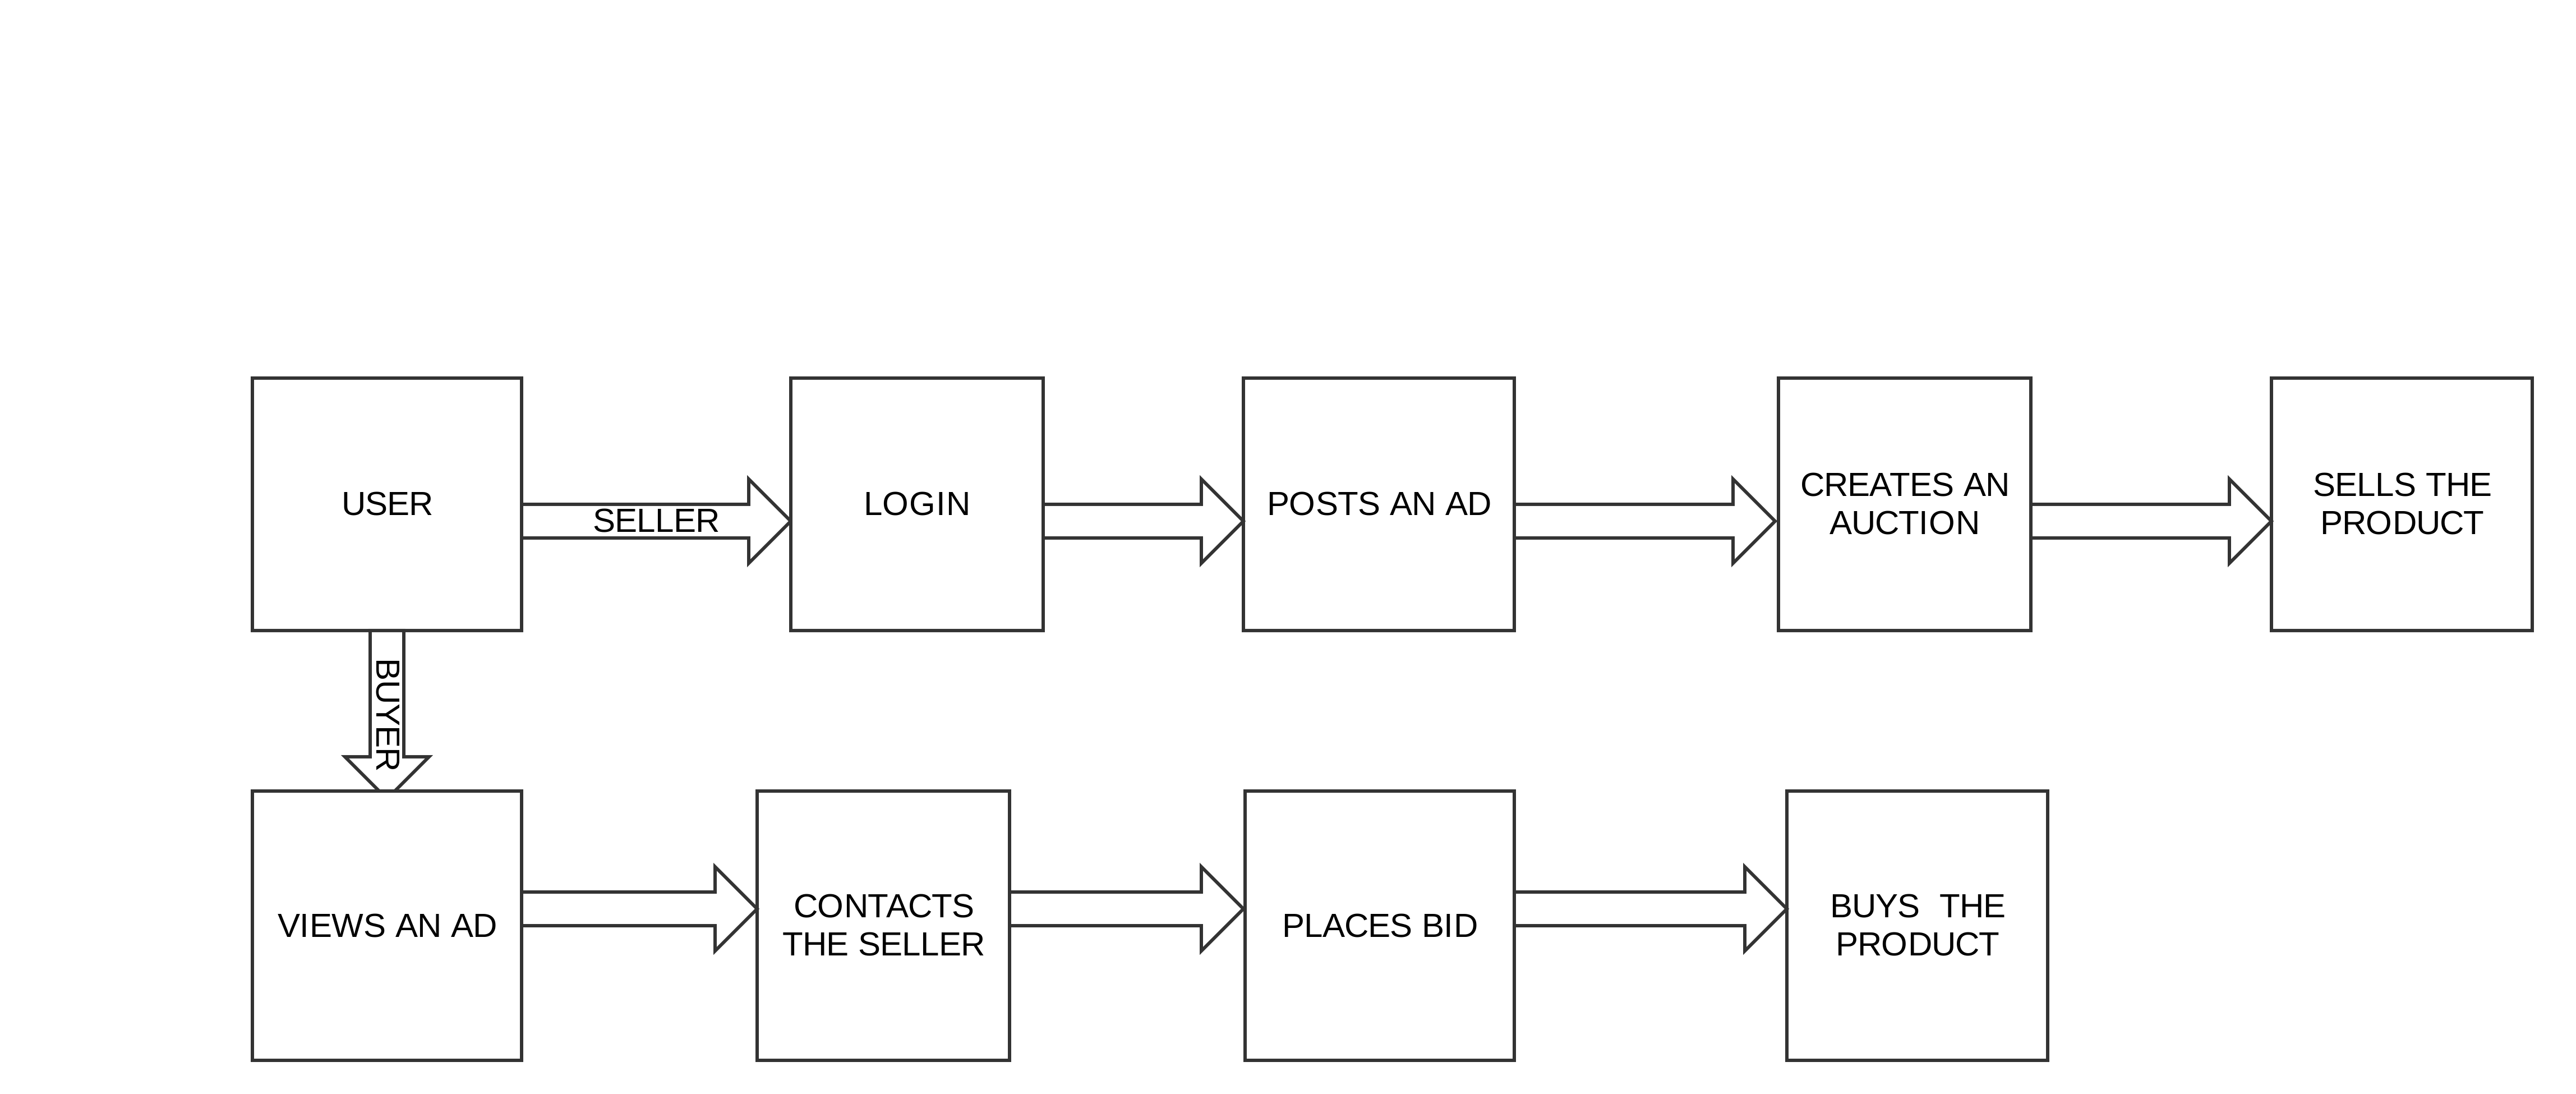
\includegraphics[width=100mm]{blockdiagram.png}
    \end{center}
\end{frame}

\begin{frame}{\huge Technology and Tools Implemented}
\begin{itemize}
\item Java Classes
\item Sevlets and JSP
\item JDBC
\item BootStrap
\item Git - Version Control
\item MVC Architecture
\begin{itemize}
\item Model - Business Logic
\item Views - Look and feel of the application
\item Controller - Translates the incoming requests to outgoing responses
\end{itemize}
\end{itemize}
\end{frame}

\begin{frame}{\huge Statistics}
\begin{center}
\begin{tabular}{ |c|c| } 
 \hline
 JSP & 18 \\ 
 Controller & 4 \\ 
 Bean Classes & 5 \\ 
 DAO & 5 \\
 Logging & 1 \\
 Filter & 1 \\
 Global Exception Handling & 1 \\
 \hline
\end{tabular}
\end{center}
\end{frame}

\begin{frame}{\huge What we have learnt}
\begin{itemize}
\item Self-learning
\item Handling errors 
\item Teamwork
\end{itemize}
\end{frame}

\begin{frame}
\begin{center}
BitBucket Demo
\end{center}
\end{frame}

\begin{frame}
\begin{center}
Application Demo
\end{center}
\end{frame}

\end{document}
